\documentclass[preprint, 3p,
authoryear]{elsarticle} %review=doublespace preprint=single 5p=2 column
%%% Begin My package additions %%%%%%%%%%%%%%%%%%%

\usepackage[hyphens]{url}

  \journal{Transportation Research Part A: Policy and
Practice} % Sets Journal name

\usepackage{graphicx}
%%%%%%%%%%%%%%%% end my additions to header

\usepackage[T1]{fontenc}
\usepackage{lmodern}
\usepackage{amssymb,amsmath}
% TODO: Currently lineno needs to be loaded after amsmath because of conflict
% https://github.com/latex-lineno/lineno/issues/5
\usepackage{lineno} % add
\usepackage{ifxetex,ifluatex}
\usepackage{fixltx2e} % provides \textsubscript
% use upquote if available, for straight quotes in verbatim environments
\IfFileExists{upquote.sty}{\usepackage{upquote}}{}
\ifnum 0\ifxetex 1\fi\ifluatex 1\fi=0 % if pdftex
  \usepackage[utf8]{inputenc}
\else % if luatex or xelatex
  \usepackage{fontspec}
  \ifxetex
    \usepackage{xltxtra,xunicode}
  \fi
  \defaultfontfeatures{Mapping=tex-text,Scale=MatchLowercase}
  \newcommand{\euro}{€}
\fi
% use microtype if available
\IfFileExists{microtype.sty}{\usepackage{microtype}}{}
\usepackage[]{natbib}
\bibliographystyle{plainnat}

\ifxetex
  \usepackage[setpagesize=false, % page size defined by xetex
              unicode=false, % unicode breaks when used with xetex
              xetex]{hyperref}
\else
  \usepackage[unicode=true]{hyperref}
\fi
\hypersetup{breaklinks=true,
            bookmarks=true,
            pdfauthor={},
            pdftitle={Framing active school travel in Ontario, or how spinach is good for you},
            colorlinks=false,
            urlcolor=blue,
            linkcolor=magenta,
            pdfborder={0 0 0}}

\setcounter{secnumdepth}{5}
% Pandoc toggle for numbering sections (defaults to be off)


% tightlist command for lists without linebreak
\providecommand{\tightlist}{%
  \setlength{\itemsep}{0pt}\setlength{\parskip}{0pt}}




\usepackage{booktabs}
\usepackage{longtable}
\usepackage{array}
\usepackage{multirow}
\usepackage{wrapfig}
\usepackage{float}
\usepackage{colortbl}
\usepackage{pdflscape}
\usepackage{tabu}
\usepackage{threeparttable}
\usepackage{threeparttablex}
\usepackage[normalem]{ulem}
\usepackage{makecell}
\usepackage{xcolor}



\begin{document}


\begin{frontmatter}

  \title{Framing active school travel in Ontario, or how spinach is good
for you}
    \author[McMaster University]{Elise Desjardins%
  %
  }
   \ead{desjae@mcmaster.ca} 
    \author[McMaster University]{Jason Lam%
  %
  }
   \ead{lamj54@mcmaster.ca} 
    \author[University of Alberta]{Darcy Reynard%
  %
  }
   \ead{reynard@ualberta.ca} 
    \author[University of Alberta]{Damian Collins%
  %
  }
   \ead{damian.collins@ualberta.ca} 
    \author[Polytechnique Montreal]{E. Owen D. Waygood%
  %
  }
   \ead{owen.waygood@polymtl.ca} 
    \author[McMaster University]{Antonio Paez%
  \corref{cor1}%
  \fnref{1}}
   \ead{paezha@mcmaster.ca} 
      \affiliation[McMaster University]{School of Earth, Environment and
Society, 1280 Main St.~W, Hamilton, Ontario, Canada L8S 4K1}
    \affiliation[University of Alberta]{Department of Earth and
Atmospheric Sciences, 1-26 Earth Sciences Building, Edmonton, Alberta,
Canada T6G 2E3}
    \affiliation[Polytechnique Montreal]{Department of Civil, Geological
and Mining Engineering, 2500, chemin de Polytechnique Montreal,
Montreal, Quebec, Canada H3T 1J4}
    \cortext[cor1]{Corresponding author}
    \fntext[1]{Corresponding author.}
  
  \begin{abstract}
  Active school travel (AST) is promoted in many jurisdictions,
  including Ontario, Canada, where there is provincial support for
  school travel planning (STP) efforts. Two pillars of school travel
  plans in the province are education and encouragement. For these
  pillars to stand, relevant stakeholders must be cognizant of and
  understand the issues and stakes. For this reason, we deem it
  important to understand how AST is communicated. In this research we
  adopt framing analysis to investigate the ways in which various
  organizations communicate to the public around AST. A frame is a
  central organizing idea or story line that provides meaning to a
  particular phenomenon, and thus helps to set the parameters for
  conversations about policy. In the case of AST, framing can influence
  what policy alternatives are perceived as available by children,
  parents, and their wider communities. The research is supported by
  natural language processing techniques applied to publicly available
  documents from Ontario stakeholders involved in school travel
  planning. We then compare the findings from these documents to a
  selection of academic studies on AST. We conclude that framing of AST
  in Ontario is mostly empirical-scientific in style, and largely in
  agreement with academic research on AST. However, it is essentially
  conservative and does not challenge the status quo of motorized
  travel. Furthermore, the frames tend to download responsibility for
  change to households, which limits the scope of policy alternatives by
  keeping collective action out of the frame.
  \end{abstract}
    \begin{keyword}
    active school travel \sep school travel planning \sep natural
language processing \sep 
    framing analysis
  \end{keyword}
  
 \end{frontmatter}

\newpage

\hypertarget{introduction}{%
\section{Introduction}\label{introduction}}

Walking and bicycling to school, commonly known as active school travel
(AST), have declined in North America for decades
\citep{rothmanDeclineActiveSchool2018}, but the appetite for these modes
is beginning to rise in many Canadian communities. For instance,
research in Toronto, Ontario found that 40\% of children who were driven
to school would like to travel by bicycle instead
\citep{laroucheRatherBikeSchool2016}. Another study in London, Ontario,
reported similar findings with respect to children's preference for
active travel \citep{larsenRouteBasedAnalysisCapture2012}. From a public
policy perspective, increasing active travel to school presents major
opportunities to improve children's health and wellbeing
\citep{faulknerActiveSchoolTransport2009}, to mitigate traffic and
improve perceptions of safety
\citep{rothmanAssociationsParentsPerception2015}, as well as to reduce
emissions and other forms of pollution
\citep{bearman2014modelling, goodman2019scenarios}.

To promote this trend, in 2017 the Government of Ontario began to
support communities develop AST initiatives through a program called
\emph{Ontario Active School Travel} (OAST). By 2021, the program, run by
\emph{Green Communities Canada} had awarded over CAD 2 million and
provided resources to over 25 projects across Ontario
\citep{GreenCommunities2016}. A popular intervention in many communities
is school travel planning (STP) \citep[see][]{GreenCommunitiesProjects}.
In this context, STPs are ``school-specific'' interventions led by a
facilitator who works with a committee of stakeholders from diverse
sectors including education, planning, transportation, and public health
to develop action plans
\citep{buliungSchoolTravelPlanning2011, mammenSchoolTravelPlanning2014}.
The five-step process involves identifying barriers to AST and
implementing solutions or activities to make AST safer and more
convenient: 1) setup of the program; 2) data collection and problem
identification; 3) action planning; 4) implementation; 5) monitoring and
evaluation \citep{hinckson2018school}.

How AST is presented to a target audience (e.g., parents or the general
public) is essential to define the parameters of what is possible
policy-wise. Drawing from concepts in communication studies, the
objective of this paper is to investigate how AST is framed in Ontario.
Gamson and Modigliani \citeyearpar{gamsonChangingCulture1987} define a
frame as a ``central organizing idea or story line that provides
meaning'' to a particular phenomenon. A frame can enable individuals
``to locate, perceive, identify, and label'' information pertaining to
various dimensions of an issue \citep{goffmanFrameAnalysisEssay1974}.
From this perspective, stakeholders involved in STP efforts play an
important role in shaping public perceptions about AST by generating
frames that create meaning, and thus influence the degree of attention
and recognition of a ``problem'' that needs to be addressed through
behavior change or new policies.

Our research is supported by natural language processing techniques,
applied to the analysis of documents produced by three STP stakeholder
groups in Ontario (municipalities, school boards, and transportation
consortia). We assemble a corpus of texts from public sources that
present information for the general public or parents who are interested
in AST and examine word frequency, bigrams, and concordances in these
selected documents. Furthermore, we use topic analysis to identify
themes presented by each stakeholder group. We then compare the findings
from these documents to a selection of studies on AST and explore the
extent to which there is concordance between the scholarly literature on
AST and materials shared with the public. The results of this analysis,
along with manual checks of the corpus by the authors, lead us to
conclude that AST is framed as a matter of individual choices instead of
collective action. The message is reasonable but inherently conservative
and it fails to communicate a sense of urgency about health and
environmental issues, which may help to explain the modest success of
related policies
\citep{buliungSchoolTravelPlanning2011, mammenSchoolTravelPlanning2014, mammenActiveSchoolTravel2014}.

\hypertarget{literature-review-ast}{%
\section{Literature Review: AST}\label{literature-review-ast}}

The desire to increase AST in Canada is warranted given its potential
physical and mental health benefits. Faulkner et al.
\citeyearpar{faulknerActiveSchoolTransport2009} concluded from their
systematic review that children who travel on foot or by bicycle to
school generally have higher levels of physical activity than their
peers who are driven to school. This relationship could be
dose-dependent, and contingent on sufficiently long trips to school to
accumulate physical activity. A walking distance of 1000-1600 metres to
school has been found to contribute to overall levels of physical
activity for boys \citep{faulknerSchoolTravelChildren2013}. The daily
routine of travelling to school can be a good opportunity for children
to regularly build physical activity into their schedule
\citep{mitraIndependentMobilityMode2013}.

More recently, the link between transport and children's wellbeing has
attracted interest too \citep{waygoodTransportChildrenWellbeing2020}.
Being driven to school reduces community interactions for children,
which may negatively impact their social wellbeing
\citep{waygoodChildrenTravelIncidental2015}. In contrast, walking and
bicycling give children opportunities to socialize
\citep{michailChildrenExperiencesTheir2021} and increase positive
emotions that contribute to wellbeing
\citep{ramanathanHappinessMotionEmotions2014a}, a feeling that children
seem to value \citep{zwertsHowChildrenView2010}. AST can also provide
opportunities for children to engage with natural environments
\citep{fuscoUnderstandingChildrenPerceptions2012, romeroChildrenExperiencesEnjoyment2015}.

Rather than describing an extensive list of factors that influence AST
and mode choice for travel to school in Canada
\citep[e.g.,][]{mammenUnderstandingDriveEscort2012, mitraIndependentMobilityMode2013, rothmanDeclineActiveSchool2018, wilsonUnderstandingChildParent2018},
we focus on two key aspects that may be targeted from a policy
perspective: built environmental factors and perceptions and behaviors
of parents.

The built environment is a key factor for physical planning, and in this
respect distance between home and school is the factor most negatively
associated with AST
\citep{ikedaAssociationsChildrenActive2018, mammenUnderstandingDriveEscort2012, pontEnvironmentalCorrelatesChildren2009, rothmanDeclineActiveSchool2018}
with less AST reported among children who have to travel farther to
school. Many studies have also found that the quality of the built
environment along the route to school and around the school site
\citep{ikedaAssociationsChildrenActive2018, rothmanActiveSchoolTransportation2021}
and provision of active travel infrastructure
\citep{chenPromotingActiveStudent2018, pontEnvironmentalCorrelatesChildren2009}
facilitate AST. Canadian youth report that they feel most safe bicycling
on streets in their neighbourhood or that have low volumes of traffic
\citep{TACbikeinfra2020}. Finally, concerns about traffic and strangers
have been reported by parents who drive their children to school
\citep{mammenUnderstandingDriveEscort2012}: ironically, concerns about
the dangers of traffic become a vicious cycle
\citep{rothmanSchoolEnvironmentStudent2017}.

Secondly, research has found that parents are key decision-makers with
respect to children's mode of travel to school
\citep{rothmanAssociationsParentsPerception2015}. Particularly, after
distance \citep{curtis2015built}, parental perceptions of the built or
school environment, as well as of their children's skills, have been
found to be key in influencing mode choice to school
\citep{demeesterParentalPerceivedNeighborhood2014, panterAttitudesSocialSupport2010, mandic2020differences, mammenUnderstandingDriveEscort2012, faulknerWhatQuickestEasiest2010}.
For example, \citet{ramanathanHappinessMotionEmotions2014a} found that
parents and children who perceived active travel as beneficial for
health and wellbeing benefits were more likely to use active modes to
get to school. Furthermore, children's mode choice to school is strongly
influenced by their parents' travel behaviors, the complexity of their
household's travel needs \citep{buliungLivingJourneySchool2021}, as well
as daily parental support \citep{mahDoesParentalSupport2017a}. This
suggests that shifting parental perceptions and habits is important.

\hypertarget{stp-frames}{%
\section{School travel planning in Canada and relevance of
frames}\label{stp-frames}}

AST has become a policy issue on the education and public health agendas
in Ontario, and is supported, albeit in a modest way, by financial
contributions from the provincial government. Still, endorsement from a
range of municipal representatives
\citep[see][]{buttazzoniSupportingActiveSchool2018, mammenPuttingSchoolTravel2015}
demonstrates that the AST issue is on the political agenda. One of the
main vehicles to promote AST is school travel planning (STP), which has
been implemented in Canada since at least the late 2000s. Within the STP
process, facilitators establish multi-sector committees which intervene
at the participating school through four pillars consisting of
\emph{{[}E{]}ducation} strategies, \emph{{[}E{]}ncouragement} through
in-person events or programs, \emph{{[}E{]}ngineering} improvements to
or around the school site, and \emph{{[}E{]}nforcement} of traffic
speeds around schools \citep[or
4Es,][]{langUnderstandingModalChoice2011, mammenActiveSchoolTravel2014}.
Of the 4Es, {[}E{]}ngineering targets the first set of factors discussed
in the preceding section (the built environment), whereas
{[}E{]}ducation and {[}E{]}ncouragement target perceptions.

The relevance of policy frames with respect to education and
encouragement is highlighted by \citet{beland2014developing}, who
remarks ``framing processes as public relations are central to policy
issues related to sustainable transportation''. Seeing how influential
parental perceptions are to AST, it is important to understand
AST-related communications, since the construction of frames for policy
positions or public issues can activate or restrict a particular
response in the intended audience
\citep{panFramingAnalysisApproach1993}. Besides parents and children,
framing can also affect broader policy support for AST in the community.
Municipal representatives are perceived to be instrumental but the
involvement of other stakeholder groups (e.g., busing consortia
representatives and local residents) can be lacking
\citep{buttazzoniSupportingActiveSchool2018}. In this sense, framing can
be used to position existing solutions as suitable to address particular
issues \citep{mahFramecriticalPolicyAnalysis2014}, which may prevent the
public from being aware of other policy approaches that challenge the
status quo. Contrariwise, framing can be instrumental to revealing more
diverse policy options than conventional wisdom would have
\citep{bosomworth2015climate}. Ultimately, it is important to understand
framing of policy issues because creating meaning through frames
contributes to the constant process of shaping our collective
understanding of issues, uncovering what we collectively find
(un)acceptable and why \citep{beland2014developing}.

Given the role of education and encouragement in STP, it is important
for the issues to be effectively framed. In the past, parents have been
found to express understandings, language, and perceptions regarding the
influence of the built environment on school travel that markedly differ
from those of planners: while parents tend to view mixed land use as
conducive for driving, transport planners see mixed uses as a key for
encouraging more active travel \citep{buliungLivingJourneySchool2021}.
Similarly mismatched understandings have been detected with respect to
factors like the convenience of different modes to school
\citep{langUnderstandingModalChoice2011}. As a consequence, STP
stakeholders must pay special attention to parents' and communities'
understanding of the decline of AST as a problem, which may affect their
receptivity to proposed solutions
\citep{buttazzoniSupportingActiveSchool2018}.

Framing is important, but not all frames are equally effective. Frames
can appeal to economic reasons, to science and logic, or to moral
obligation. For example, \citet{severson2015moral} report that overall
support for climate change policy increases more when scientific frames,
secular moral frames, and economic equity frames are used, compared to
economic efficiency or religious moral frames. Frames can also be
positive or negative, and there is evidence that negative framing may be
more effective at motivating individuals, for example, to change
transport modes to reduce CO2 emissions
\citep{waygoodCO2ValenceFraming2018}. As well, the effectiveness of the
framing depends on the psychological distance to the relevant issues:
how socially, temporally, geographically, or hypothetically close an
individual perceives themselves to the issues can affect their support
for various policies \citep{maiella2020psychological}. For this reason,
stakeholders involved in STP must make conscious choices about how
issues surrounding AST are communicated if the goal is to increase
support for and buy-in of AST policies.

\hypertarget{data}{%
\section{Data}\label{data}}

\hypertarget{data-retrieval}{%
\subsection{Data retrieval}\label{data-retrieval}}

\hypertarget{policy-documents}{%
\subsubsection{Policy documents}\label{policy-documents}}

We assembled a collection of publicly available documents that were
sourced online from the main stakeholder groups involved in STP
initiatives in Ontario: i) school boards (public or Catholic and
English-speaking only); ii) municipal governments; and iii)
transportation consortia. The latter involve collaborations between
municipal regions and school boards to deliver more efficient and timely
regional transportation services to schools. Non-profit organizations,
police services, and advocacy groups are other stakeholders who often
play a role in supporting AST and/or STP, but this study does not
include any documents from these groups because they do not consistently
participate in STP initiatives in Ontario.

The search was guided first by a list of all English public and Catholic
school boards across Ontario. The websites of each school board were
manually searched for pages related to school transport or travel. Any
pages relevant to these topics were downloaded. Next, we searched
municipal government and transportation consortia websites. These were
identified based on geographic area. Likewise, webpages related to
active transport or school travel were downloaded.

Webpages from STP stakeholder groups were included in our analysis if
they were findable. This primary criterion was important since our
analysis pertains communication of issues to the general public. Thus,
we included only webpages that were readily accessible, which we defined
as requiring no more than four links from the initial Google search to
reach.

The initial corpus of documents from STP stakeholder groups included 69
relevant webpages. We refer to these as policy+practice documents
throughout the paper. It is important to note that school boards,
municipalities, and transportation consortia may or may not publish
information about their involvement in AST and STP efforts on their
respective websites or in policy documents. Search results are
summarized in Table \ref{tab:policy-documents}.

\begin{table}

\caption{\label{tab:policy-documents}\label{tab:search-results}Search results from the main STP stakeholder groups.}
\centering
\begin{tabular}[t]{>{}l|l|>{}l}
\toprule
Stakeholder & Total & Retrieved\\
\midrule
\cellcolor{gray!6}{\textbf{School boards}} & \cellcolor{gray!6}{62} & \cellcolor{gray!6}{32}\\
\textbf{Municipalities} & 62 & 28\\
\cellcolor{gray!6}{\textbf{Transportation consortia}} & \cellcolor{gray!6}{39} & \cellcolor{gray!6}{9}\\
\bottomrule
\end{tabular}
\end{table}

\hypertarget{academic-papers}{%
\subsubsection{Academic papers}\label{academic-papers}}

We conducted a search on Web of Science for scholarly papers on the
topic of school travel using Web of Science's Core Collection. The
search was conducted in the Winter of 2021 and the parameters used were
\{active OR walk* or cycl* or bicycl*\} AND \{``school travel''\}.
Initially, we found 322 papers, which we reduced to 250 after selecting
only papers in the fields of transportation, planning, urban studies,
geography, and public health. These fields were chosen because they had
the greatest volume of documents and/or were of disciplinary interest to
the authors. This list with 250 documents was then manually curated by
the authors to ensure that all documents were relevant. This was done by
checking the title and reading the abstract of the papers. For example,
a paper with the title ``Impact of automated photo enforcement of
vehicle speed in school zones'' \citep{quistberg2019impact} was excluded
as being tangential to our research; the abstract of another paper
revealed that it was mainly concerned with survey methods: ``Common
methods for measuring mode share include Hands Up surveys and family
surveys, but these require teacher and parental involvement.''
\citep{sersli2019getting}. After this process, our academic corpus
comprised 227 journal articles that were readied for analysis.

\hypertarget{data-cleaning}{%
\subsection{Data cleaning}\label{data-cleaning}}

A multi-step process was conducted to ensure that the analysis captured
as much text as possible from both the policy documents (n = 64) and
academic papers (n = 227). Webpages were manually downloaded in portable
document format (PDF) and trimmed so that pages that only consisted of
tables, figures, or references were removed. After converting into
\texttt{txt} files and importing for analysis, we manually removed any
remaining tables, figures, references, headers/footings, and captions
that could not be trimmed. We also manually removed any extraneous
material that did not pertain to AST specifically (e.g., references,
footnotes, weblinks, etc.). In the final step, we removed all blank
spaces, punctuation, capitalization, and numbers. English stop words
(i.e., words such as \emph{and} or \emph{the}) and other frequent terms
in the documents like ``school'' and specific location names were
removed from the corpora.

\hypertarget{methods}{%
\section{Methods}\label{methods}}

\hypertarget{process-of-framing-analysis}{%
\subsection{Process of Framing
Analysis}\label{process-of-framing-analysis}}

Topic modelling was used to analyze the documents retrieved. This is a
natural language processing technique used to analyze text to identify
the language and concepts being communicated. This method is practical
for researchers working with large amounts of text because it can assist
and complement the manual coding of topics that would normally take
place to analyze or summarize textual data
\citep{jacobiQuantitativeAnalysisLarge2016}. We primarily use the
following \texttt{R} packages: \texttt{tidytext}
\citep{silge2016tidytext}, \texttt{topicmodels} \citep{grun2011topic},
\texttt{word2vec} \citep{wijffels2021word2vec}, and \texttt{wordcloud}
\citep{fellows2018wordloud}.

We estimate latent Dirichlet allocation (LDA) models to identify topics
contained in both the STP and academic documents. The model's output is
``a set of topics consisting of clusters of words that co-occur in these
documents according to certain patterns''
\citep{jacobiQuantitativeAnalysisLarge2016}. Researchers must then
interpret the identified topics, as done after other methods of manual
coding.

\hypertarget{reproducibility}{%
\subsection{Reproducibility}\label{reproducibility}}

This paper is an example of open and reproducible research that uses
only open software. The source document is an R markdown document.
Following best practices in spatial data science
\citep{brunsdon2020opening}, the code and data needed to reproduce our
research or conduct a similar analysis for other regions are available
in a publicly available repository\footnote{\url{https://github.com/desjae/AST-Framing-Analysis-Ontario}}.

\hypertarget{results}{%
\section{Results}\label{results}}

\hypertarget{word-and-document-frequency}{%
\subsection{Word and document
frequency}\label{word-and-document-frequency}}

We analyzed word and document frequency for each corpus of text. Table
\ref{tab:word-table} shows the most frequent terms found in the
municipal, transportation consortia, school board, and academic
documents. Policy documents and academic papers reference \emph{active},
\emph{travel}, \emph{walking}, \emph{biking} or \emph{cycling}, and
\emph{students} more than other terms. Each corpus also has
\emph{safety} and \emph{traffic} as common words, which suggests that
these are common concerns. The word \emph{physical} is present in each
corpus, but this could refers to \emph{physical activity} or the
\emph{physical environment}. Furthermore, documents from STP stakeholder
groups discuss \emph{resources}, \emph{information}, and \emph{services}
about school travel. Unlike the academic papers, policy+practice
documents frequently include the words \emph{route} or \emph{routes}.
This could indicate the role of STP stakeholder groups in identifying
safe routes to school to share with parents or families. In the section
below, the context in which these terms are used is explored further.

The academic corpus differs from the policy documents in that
\emph{parents} and \emph{distance} are the second and third most common
terms. In addition, \emph{time}, \emph{factors}, \emph{environment}, and
\emph{age} are also identified in the academic papers. The prevalence of
these terms is consistent with an academic focus on exploring the
variables that influence travel to school. These words are absent from
the list of common words in policy+practice documents. Table
\ref{tab:word-table} indicates that the academic corpus discusses a
broader range of determinants of AST than the policy documents. The
number of references for each term in the academic papers is also
substantially higher due to the inclusion of more documents.

\begin{table}

\caption{\label{tab:word-table}\label{tab:word-table}Top 25 terms identified in each corpus. Document frequencies are also indicated.}
\centering
\resizebox{\linewidth}{!}{
\begin{tabular}[t]{lcclcclcclcc}
\toprule
\multicolumn{3}{c}{Municipalities} & \multicolumn{3}{c}{School Boards} & \multicolumn{3}{c}{Transportation Consortia} & \multicolumn{3}{c}{Academic Papers} \\
\cmidrule(l{3pt}r{3pt}){1-3} \cmidrule(l{3pt}r{3pt}){4-6} \cmidrule(l{3pt}r{3pt}){7-9} \cmidrule(l{3pt}r{3pt}){10-12}
Term & Count (n) & Documents (n) & Term & Count (n) & Documents (n) & Term & Count (n) & Documents (n) & Term & Count (n) & Documents (n)\\
\midrule
\cellcolor{gray!6}{active} & \cellcolor{gray!6}{248} & \cellcolor{gray!6}{26} & \cellcolor{gray!6}{active} & \cellcolor{gray!6}{124} & \cellcolor{gray!6}{13} & \cellcolor{gray!6}{active} & \cellcolor{gray!6}{67} & \cellcolor{gray!6}{7} & \cellcolor{gray!6}{walking} & \cellcolor{gray!6}{5059} & \cellcolor{gray!6}{220}\\
travel & 126 & 20 & bus & 120 & 20 & walking & 55 & 8 & parents & 3927 & 209\\
\cellcolor{gray!6}{walking} & \cellcolor{gray!6}{90} & \cellcolor{gray!6}{25} & \cellcolor{gray!6}{travel} & \cellcolor{gray!6}{103} & \cellcolor{gray!6}{11} & \cellcolor{gray!6}{walk} & \cellcolor{gray!6}{49} & \cellcolor{gray!6}{8} & \cellcolor{gray!6}{distance} & \cellcolor{gray!6}{3252} & \cellcolor{gray!6}{203}\\
bike & 87 & 15 & information & 65 & 21 & travel & 41 & 8 & students & 2956 & 171\\
\cellcolor{gray!6}{cycling} & \cellcolor{gray!6}{78} & \cellcolor{gray!6}{22} & \cellcolor{gray!6}{walking} & \cellcolor{gray!6}{57} & \cellcolor{gray!6}{17} & \cellcolor{gray!6}{students} & \cellcolor{gray!6}{39} & \cellcolor{gray!6}{9} & \cellcolor{gray!6}{cycling} & \cellcolor{gray!6}{2739} & \cellcolor{gray!6}{170}\\
\addlinespace
safety & 71 & 21 & walk & 53 & 13 & safety & 32 & 6 & environment & 2585 & 200\\
\cellcolor{gray!6}{health} & \cellcolor{gray!6}{65} & \cellcolor{gray!6}{21} & \cellcolor{gray!6}{weather} & \cellcolor{gray!6}{40} & \cellcolor{gray!6}{11} & \cellcolor{gray!6}{help} & \cellcolor{gray!6}{29} & \cellcolor{gray!6}{9} & \cellcolor{gray!6}{traffic} & \cellcolor{gray!6}{2334} & \cellcolor{gray!6}{206}\\
physical & 63 & 18 & safety & 40 & 19 & schools & 25 & 9 & choice & 2295 & 167\\
\cellcolor{gray!6}{traffic} & \cellcolor{gray!6}{59} & \cellcolor{gray!6}{20} & \cellcolor{gray!6}{safe} & \cellcolor{gray!6}{39} & \cellcolor{gray!6}{19} & \cellcolor{gray!6}{children} & \cellcolor{gray!6}{25} & \cellcolor{gray!6}{6} & \cellcolor{gray!6}{activity} & \cellcolor{gray!6}{2265} & \cellcolor{gray!6}{207}\\
road & 56 & 13 & services & 37 & 17 & community & 24 & 7 & physical & 2238 & 213\\
\addlinespace
\cellcolor{gray!6}{activity} & \cellcolor{gray!6}{55} & \cellcolor{gray!6}{14} & \cellcolor{gray!6}{planning} & \cellcolor{gray!6}{37} & \cellcolor{gray!6}{7} & \cellcolor{gray!6}{bus} & \cellcolor{gray!6}{18} & \cellcolor{gray!6}{4} & \cellcolor{gray!6}{trips} & \cellcolor{gray!6}{2164} & \cellcolor{gray!6}{168}\\
schools & 52 & 14 & parents & 32 & 17 & route & 17 & 5 & car & 2140 & 193\\
\cellcolor{gray!6}{children} & \cellcolor{gray!6}{47} & \cellcolor{gray!6}{15} & \cellcolor{gray!6}{sustainable} & \cellcolor{gray!6}{31} & \cellcolor{gray!6}{8} & \cellcolor{gray!6}{zone} & \cellcolor{gray!6}{16} & \cellcolor{gray!6}{6} & \cellcolor{gray!6}{safety} & \cellcolor{gray!6}{2111} & \cellcolor{gray!6}{202}\\
plan & 45 & 16 & children & 31 & 14 & resources & 16 & 6 & time & 2091 & 216\\
\cellcolor{gray!6}{students} & \cellcolor{gray!6}{44} & \cellcolor{gray!6}{14} & \cellcolor{gray!6}{child} & \cellcolor{gray!6}{31} & \cellcolor{gray!6}{12} & \cellcolor{gray!6}{day} & \cellcolor{gray!6}{16} & \cellcolor{gray!6}{4} & \cellcolor{gray!6}{factors} & \cellcolor{gray!6}{2083} & \cellcolor{gray!6}{214}\\
\addlinespace
walk & 43 & 18 & day & 29 & 13 & safe & 15 & 5 & child & 2060 & 185\\
\cellcolor{gray!6}{public} & \cellcolor{gray!6}{39} & \cellcolor{gray!6}{15} & \cellcolor{gray!6}{routes} & \cellcolor{gray!6}{28} & \cellcolor{gray!6}{14} & \cellcolor{gray!6}{planning} & \cellcolor{gray!6}{15} & \cellcolor{gray!6}{4} & \cellcolor{gray!6}{walk} & \cellcolor{gray!6}{1985} & \cellcolor{gray!6}{198}\\
community & 37 & 19 & physical & 28 & 11 & physical & 15 & 7 & public & 1973 & 206\\
\cellcolor{gray!6}{safe} & \cellcolor{gray!6}{34} & \cellcolor{gray!6}{16} & \cellcolor{gray!6}{health} & \cellcolor{gray!6}{28} & \cellcolor{gray!6}{11} & \cellcolor{gray!6}{healthy} & \cellcolor{gray!6}{14} & \cellcolor{gray!6}{6} & \cellcolor{gray!6}{age} & \cellcolor{gray!6}{1774} & \cellcolor{gray!6}{209}\\
benefits & 32 & 17 & inclement & 25 & 11 & traffic & 13 & 6 & urban & 1749 & 198\\
\addlinespace
\cellcolor{gray!6}{play} & \cellcolor{gray!6}{31} & \cellcolor{gray!6}{2} & \cellcolor{gray!6}{eligibility} & \cellcolor{gray!6}{24} & \cellcolor{gray!6}{11} & \cellcolor{gray!6}{support} & \cellcolor{gray!6}{13} & \cellcolor{gray!6}{6} & \cellcolor{gray!6}{different} & \cellcolor{gray!6}{1695} & \cellcolor{gray!6}{213}\\
resources & 30 & 13 & consortium & 24 & 9 & families & 13 & 5 & home & 1691 & 197\\
\cellcolor{gray!6}{healthy} & \cellcolor{gray!6}{29} & \cellcolor{gray!6}{16} & \cellcolor{gray!6}{region} & \cellcolor{gray!6}{23} & \cellcolor{gray!6}{10} & \cellcolor{gray!6}{way} & \cellcolor{gray!6}{12} & \cellcolor{gray!6}{5} & \cellcolor{gray!6}{social} & \cellcolor{gray!6}{1672} & \cellcolor{gray!6}{189}\\
routes & 27 & 13 & service & 22 & 11 & student & 12 & 5 & significant & 1644 & 206\\
\cellcolor{gray!6}{lanes} & \cellcolor{gray!6}{26} & \cellcolor{gray!6}{3} & \cellcolor{gray!6}{•} & \cellcolor{gray!6}{21} & \cellcolor{gray!6}{1} & \cellcolor{gray!6}{region} & \cellcolor{gray!6}{12} & \cellcolor{gray!6}{4} & \cellcolor{gray!6}{mobility} & \cellcolor{gray!6}{1634} & \cellcolor{gray!6}{136}\\
\bottomrule
\multicolumn{12}{l}{\rule{0pt}{1em}\textit{Note: }}\\
\multicolumn{12}{l}{\rule{0pt}{1em} }\\
\multicolumn{12}{l}{\rule{0pt}{1em}\textsuperscript{a} Count (n) refers to the total number of times the term is found in the corpora}\\
\multicolumn{12}{l}{\rule{0pt}{1em}\textsuperscript{b} Documents (n) refers to the total number of documents that feature the term}\\
\end{tabular}}
\end{table}

Examination of document frequency reveals terms that are not present in
all policy documents. This suggests that although documents pertain to
school travel, not all stakeholders across Ontario disseminate
information about AST. We manually searched the policy+practice corpus
and found that 48\% of documents mention AST and 16\% mention STP. In
contrast, inclement weather and its impacts on busing is a common topic
addressed in school board and transportation consortia documents.

\hypertarget{bigrams-and-concordances}{%
\subsection{Bigrams and concordances}\label{bigrams-and-concordances}}

\begin{figure}

{\centering 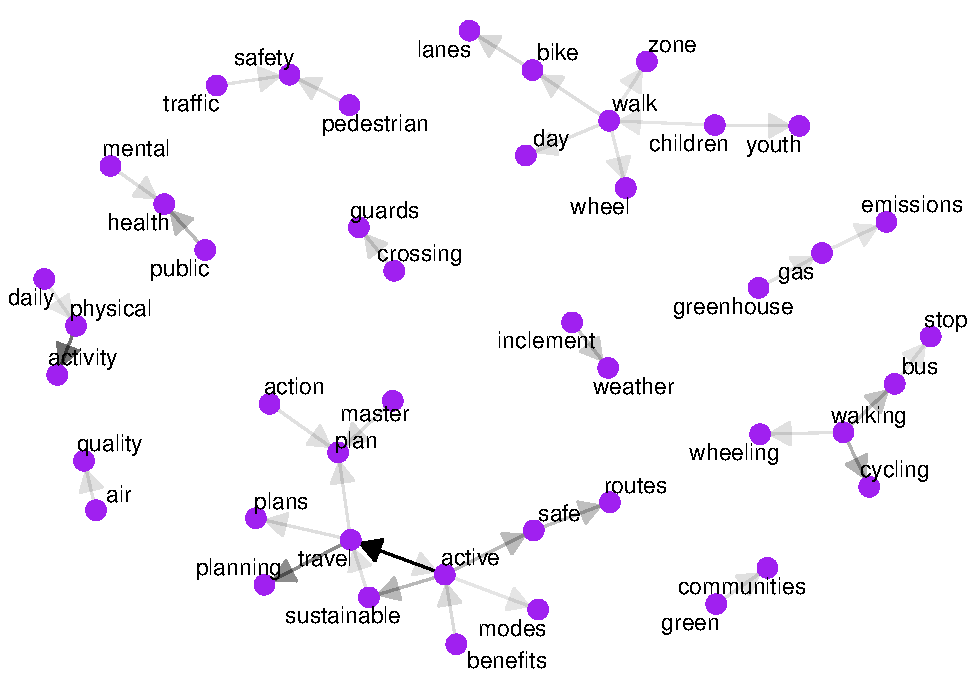
\includegraphics[width=1\linewidth]{AST-Framing-Ontario_files/figure-latex/policy-visual-1} 

}

\caption{\label{fig:policy-visual}Most common bigrams found across all policy documents (i.e., school board, municipality, and transportation consortia combined).}\label{fig:policy-visual}
\end{figure}

Bigrams refer to pairs of consecutive words. We combined all
municipality, school board, and transportation consortia documents into
the policy+practice corpus. Figure \ref{fig:policy-visual} shows all of
the bigrams that occur more than 10 times in this corpus. This figure
highlights the main ideas that are presented to the public in each of
the policy corpora. The directional arrows indicate the arrangement of
the words (e.g., active travel and not travel active) and the colour
gradient of the arrows corresponds to the most frequently mentioned
pairs (e.g., bigrams with darker arrows are found in the corpus more
often).

STP stakeholders discuss \emph{physical activity} and \emph{public
health} in the context of AST. In addition, \emph{travel planning},
\emph{bike lanes}, and \emph{safe routes} are also identified,
conceivably as either proposed solutions or built environment factors
that support AST. Key issues related to transport such as \emph{traffic
safety}, \emph{air quality}, and \emph{greenhouse gases} are conveyed to
the public through these policy documents. It is not surprising to find
this focus given that municipalities in Ontario are concerned about
climate change and have increasingly looked to active travel to offset
transport-related emissions in urban areas. We also found \emph{mental
health}, \emph{walk zone}, and \emph{green communities} as common pairs
of consecutive words. The latter makes sense given the involvment of
\emph{Green Communities Canada} in AST initiatives in Ontario. Overall,
the policy documents from STP stakeholder groups seem to focus on four
key areas: i) benefits or impacts of AST; ii) mechanisms of
intervention; iii) concerns or barriers; and iv) supports for AST. This
interpretation indicates that the general public accessing information
about AST in Ontario is informed about a wide range of content related
to this issue.

Next, we analyzed bigrams in the academic corpus separately to compare
with the policy+practice corpus. Figure \ref{fig:academic-visual}
indicates that academic papers include several common bigrams that were
also found in the policy documents including \emph{physical activity},
which is the top bigram, as well as \emph{traffic safety} and \emph{safe
routes}. However, many other factors are identified in the academic
corpus that are not presented to the general public through policy
documents. Terms like \emph{built environment}, \emph{independent
mobility}, and \emph{urban form} are examples of these factors. Academic
papers also often discuss \emph{distance home}, \emph{car ownership},
\emph{household income}, and \emph{population density}, which are
factors that have been found to influence AST. Finally, the presence of
\emph{statistically significant} among the top bigrams indicates that
researchers often aim to identify associations using statistical
measures. We found that the academic corpus focuses on a greater range
of topics than found in the policy+practice documents.

\begin{figure}

{\centering 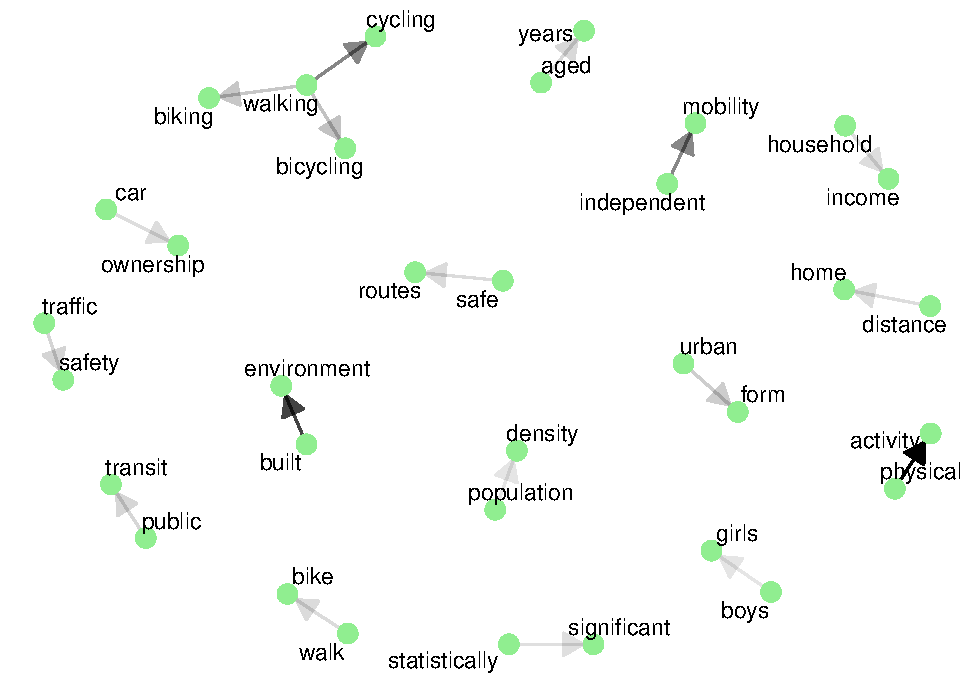
\includegraphics[width=1\linewidth]{AST-Framing-Ontario_files/figure-latex/academic-visual-1} 

}

\caption{\label{fig:academic-visual}Most common bigrams found in the academic papers.}\label{fig:academic-visual}
\end{figure}

We interpreted the most common bigrams from the policy+practice corpus
(see Figure \ref{fig:policy-visual}) as the main ideas that STP
stakeholder groups focus on and communicate to the public about AST. We
then examined the context of these key ideas by extracting
words-in-context from the corpora. Table \ref{tab:policy-concordance}
presents some examples from select policy documents that illustrate how
the most common bigrams are communicated to the public.

\begin{table}

\caption{\label{tab:content-table}\label{tab:policy-concordance}The context of key terms that were identified as common bigrams.}
\centering
\begin{tabular}[t]{>{}ll>{\raggedright\arraybackslash}p{20em}}
\toprule
Terms & Stakeholder & Context\\
\midrule
\textbf{\cellcolor{gray!6}{Air Quality}} & \cellcolor{gray!6}{School Board} & \cellcolor{gray!6}{Active transportation [...] improves air quality.}\\
\textbf{Benefit} & Municipality & Stronger bones and muscles, improved self-esteem and sense of well-being while reducing stress and risk of chronic disease all benefit those who use active transportation.\\
\textbf{\cellcolor{gray!6}{Walking School Bus}} & \cellcolor{gray!6}{School Board} & \cellcolor{gray!6}{While taking part in a walking school bus, your child will enjoy seeing friends on the way to school. They will be active more often. This is also a great opportunity for your child to socialize with school friends in a monitored and safe way where they can practice social distancing, modelled by a leader.}\\
\textbf{Community} & School Board & Help your students get started on the right foot - encourage them to walk or bike to school when possible. Even leaving the car a block or two and walking the rest of the way helps. It’s good for the environment and your health, and teaches your child independence and community awareness.\\
\textbf{\cellcolor{gray!6}{Emissions}} & \cellcolor{gray!6}{Consortia} & \cellcolor{gray!6}{An active school commute also reduces congestion in school zones and contributes to reducing greenhouse gas emissions – it’s a win-win for everyone!}\\
\addlinespace
\textbf{Health} & Municipality & Active School Travel allows school-aged children the chance to participate in moderate to intense physical activity. This is linked with lower body mass index and improved cardiovascular health.\\
\textbf{\cellcolor{gray!6}{Lanes}} & \cellcolor{gray!6}{Municipality} & \cellcolor{gray!6}{We are continuing to build on the cycling and pedestrian network by adding more bike lanes, building multi-use paths and encouraging developments to provide better pedestrian/cycling environments.}\\
\textbf{Mental Health} & Municipality & Active and Sustainable School Travel (ASST) not only improves physical and mental health but contributes to a healthier environment and safer streets.\\
\textbf{\cellcolor{gray!6}{Physical Health}} & \cellcolor{gray!6}{Municipality} & \cellcolor{gray!6}{Encouraging Active Transportation promotes physical health and recreation, helps manage congestion, reduces emissions and supports municipal objectives for efficient land use.}\\
\bottomrule
\end{tabular}
\end{table}

\hypertarget{topic-modelling}{%
\subsection{Topic modelling}\label{topic-modelling}}

\begin{figure}
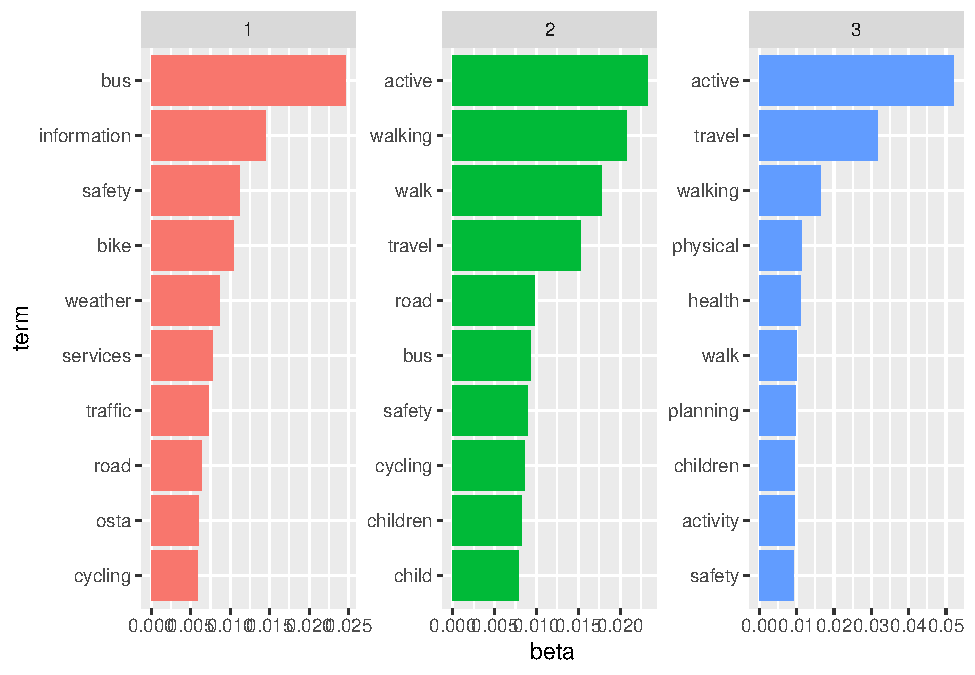
\includegraphics[width=1\linewidth]{AST-Framing-Ontario_files/figure-latex/policy-terms-1} \caption{\label{fig:policy-terms}Topics identified in the policy+practice corpus according to clusters of words. The per-word-per-topic probabilities are shown by beta.}\label{fig:policy-terms}
\end{figure}

\begin{figure}
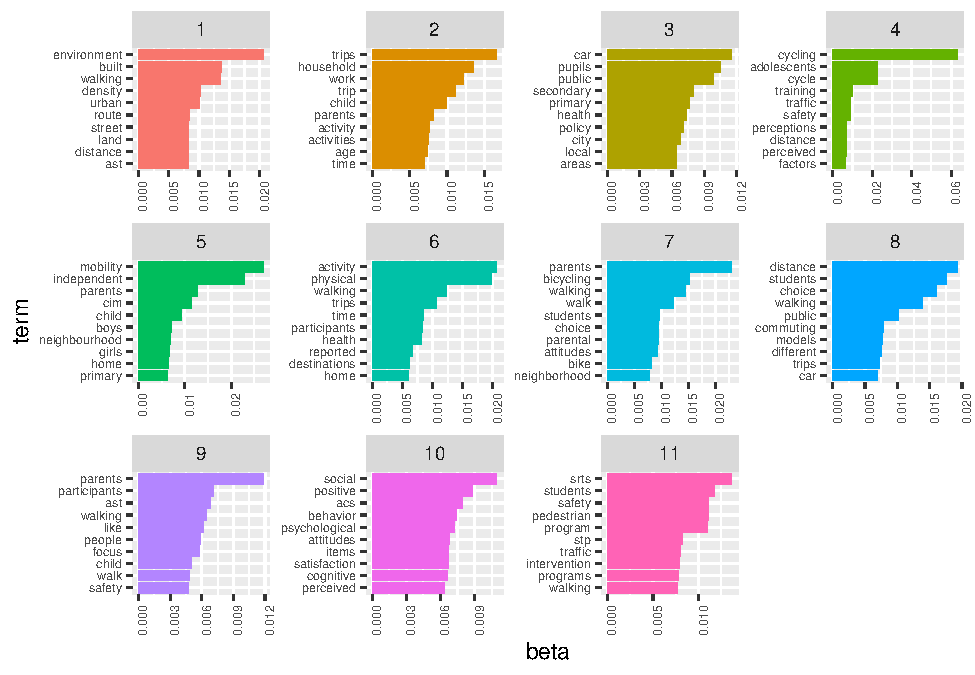
\includegraphics[width=1\linewidth]{AST-Framing-Ontario_files/figure-latex/academic-terms-1} \caption{\label{fig:academic-terms}Topics identified in the academic corpus according to clusters of words. The per-word-per-topic probabilities are shown by beta.}\label{fig:academic-terms}
\end{figure}

We conducted topic modelling to examine the different topics found in
the policy+practice and academic corpora. We estimated Latent Dirichlet
Allocation (LDA) models for each corpus. Parameter tuning suggests that
the policy+practice corpus has between 9 and 13 topics and the academic
corpus has between 17 and 25 topics. After running the LDA model for the
academic corpus, we realized the difficulty of interpreting as many as
17 topics based on the clusters of words that were identified. We
experimented with the model by adjusting the number of topics and
evaluating the output of terms in each topic. We found that there were 9
distinct topics that could be interpreted in the policy+practice corpus
and 11 topics in the academic corpus, after which there was too much
overlap for the clusters to be meaningfully distinguished. Figures
\ref{fig:policy-terms} and \ref{fig:academic-terms} present the main
terms associated with the topics found in each corpus.

In the policy+practice corpus, we identified the following topics based
on the cluster of words: (1) safety; (2) weather and busing; (3) active
travel planning; (4) walking; (5) resources for walking; (6) bicycling;
(7) active travel concerns; (8) benefits of active travel; and (9)
busing logistics. These topics indicate that STP stakeholder groups are
sending the message that walking and bicycling to school are healthy
travel modes for students, particularly in terms of physical activity.
We also found that information is shared to support parents and students
in using active modes to school, for example regarding the availability
of bicycling lanes and tips for route choice for walking.

The academic corpus has a higher number of topics likely due to the
volume of papers included. The following topics were identified based on
the clusters of words: (1) physical activity; (2) safe routes to school
for active travel; (3) behaviors and attitudes; (4) bicycling; (5)
walking; (6) built environment; (7) trip choice; (8) active school
travel interventions; (9) parents; (10) children's independent mobility;
and (11) public health and policies. This corpus reflects a broader
range of topics than the policy+practice corpus.

\hypertarget{frames}{%
\subsection{Frames}\label{frames}}

Based on the identified bigrams and topics, we determined that the
policy+practice corpus primarily frames AST as a health and
environmental issue. STP stakeholder groups appear to position walking,
bicycling, or rolling to school as beneficial to individual health, via
physical activity and improved mental health, and to the broader
community through a reduction in traffic and vehicle emissions. Here, we
present an example that illustrates how the health and environmental
frame is communicated:

\begin{quote}
\emph{Active school travel is a great way for children to be physically
active, which is associated with improved physical and mental health,
while making school zones safer, by reducing traffic volumes at and
around schools.}(Region of Leeds, Grenville and Lanark)
\end{quote}

Furthermore, we found that policy documents make claims about the
benefits of AST that are consistent with the findings of academic
research and evaluation.

\begin{quote}
\emph{There are lots of benefits in the classroom for children that walk
or cycle to school on a regular basis. Some of these benefits include
improved concentration and better coping with stress. Being outside
helps to prevent feelings of isolation and increases their social
interactions. Walking and biking to school can also save you money and
lead to fewer cars on the road.} (City of Ottawa)
\end{quote}

The secondary frame in policy documents is that AST is accessible and
feasible for children and parents. Despite the emphasis on the logistics
of busing in the topic modelling, the documents indicate that there is
an opportunity for or prospect of behavior change. Some cities and
schools explain how children and parents can leave the car at home and
make the journey to school on foot or by bike. This frame encourages the
public to evaluate their own travel decisions and to access resources
(e.g., walking skills checklist) that will help them make AST a first
choice. Examples of this secondary frame include:

\begin{quote}
\emph{Help your students get started on the right foot - encourage them
to walk or bike to school when possible. Even leaving the car a block or
two and walking the rest of the way helps. It's good for the environment
and your health, and teaches your child independence and community
awareness.} (Halton District School Board)
\end{quote}

Finally, both frames present the benefits of AST. STP stakeholder groups
seem to be communicating that AST is a healthy and accessible option as
a result of school travel plans and improvements to the built
environment. This could include examples of various efforts that are
underway to support AST including route planning.

\begin{quote}
\emph{School Travel Planning is a community-based approach that aims to
increase the number of students and adults choosing active and
sustainable travel to get to and from school. This approach addresses
concerns about safety, physical activity, and the environment.} (City of
Hamilton)
\end{quote}

Beyond supporting communities to develop STPs, these frames tend to
place responsibility for change squarely on the members of the
community:

\begin{quote}
\emph{A way to make sure your child is safe while walking to school is
with a `walking school bus.' Here are some tips for a walking
schoolbus\ldots{[}tips{]}\ldots Have fun!} (City of Ottawa)
\end{quote}

\hypertarget{discussion}{%
\section{Discussion}\label{discussion}}

\hypertarget{current-ast-frames-in-ontario}{%
\subsection{Current AST frames in
Ontario}\label{current-ast-frames-in-ontario}}

In Ontario, municipalities, school boards and transportation consortia
do not consistently include AST in their public communications. Indeed,
as noted above, less than 50\% of documents from these organizations
discuss AST. Interpretation of the text assisted by natural language
processing reveals that when AST is discussed, the primary frame
emphasizes its benefits to the health and wellbeing of both children and
the environment. The policy documents reflect the evidence that AST
contributes positively to children's physical health
\citep[see][]{faulknerActiveSchoolTransport2009, schoeppeAssociationsChildrenActive2015},
although the statements regarding the benefits of AST to children's
school performance are less well-supported in the extant literature
\citep{westmanTravelChildWellbeing2020}. STP stakeholder groups also
communicate that increasing AST may reduce traffic near and around
schools. This is conveyed presumably to alleviate parental concerns
about traffic and safety
\citep{eversParentSafetyPerceptions2014, mammenUnderstandingDriveEscort2012, rothmanAssociationsParentsPerception2015, wilsonUnderstandingChildParent2018}
or to reduce the frequency of risky behaviors from drivers around
schools \citep{rothmanSchoolEnvironmentStudent2017}.

In the secondary frame, AST is presented as an accessible and feasible
way for children to travel to and from school. Children and parents are
encouraged to adopt new travel behaviors. STP stakeholder groups
identified different ways that parents could encourage or support their
children to commute to school by using active modes (e.g., walking tip
sheets, walking school buses, etc.). The general emphasis of this frame
is communicating information that could change parental perceptions
about the ease of their children using active modes to school, which may
be seen by STP stakeholder groups as a ``modifiable'' factor
\citep[see][]{riaziCorrelatesChildrenIndependent2019}. In turn, this
could encourage parents to modify their routines and incorporate
opportunities for their children to use active modes to school.

Both frames present AST in a positive light, by highlighting the
potential benefits. However, neither frame appears to explain why
declining rates of AST are a problem or convey any urgency to this issue
so that it attracts the attention of parents, the general public, or
policy makers. For example, parents who drive their children to school
have reported concerns about traffic volume around schools
\citep{mammenUnderstandingDriveEscort2012}, but may not recognize that
their own behavior contributes to the problem that is perceived to
prevent their child from safely walking or bicycling to school
\citep{collinsSafeJourneysEnterprising2001, rothmanSchoolEnvironmentStudent2017}.
There is evidence that negative framing is more effective at eliciting
responses than positive framing
\citep[e.g.,][]{kahneman1979interpretation, waygoodCO2ValenceFraming2018}.
In this case, the frames emphasize the positive side of active travel
but leave the negative impacts of behaviors such driving children to
school out of the frame.

Further, behavior change is mainly presented as an option for some but
not an imperative for all, which keeps collective action through
government entities out of the frame. This echoes the findings of
Reynard et al. \citeyearpar{reynardGrowthResilienceHow2021}, who found
in their analysis of Canadian municipal documents that one of the
dominant frames was to present behaviors that help mitigate the climate
crisis as an individual choice but not ``the expected norm'', or what
society approves of, i.e., an injunctive norm
\citep{lapinski2005explication}. In this case, a stronger case of
society's disapproval remains to be made.

Overall, we find that the proposed solutions in the secondary frame
reinforce some of the same ideas: 1) behavior change from households
making different travel decisions (individual responsibility); 2)
policies that create resources for AST (mainly through education and
planning); and 3) engineering solutions like bicycle lanes. This
reflects findings from the AST literature that a range of solutions are
needed to address different factors that influence AST
\citep[\emph{inter alia,
see}][]{mitraIndependentMobilityMode2013, panterAttitudesSocialSupport2010}.
The recognition of engineering changes may reflect the strong engagement
of engineering staff and municipal representatives in the Canadian STP
process
\citep{buttazzoniSupportingActiveSchool2018, mammenPuttingSchoolTravel2015},
as well as the evidence that the built environment influences mode
choice to school. However, these measures tend to support the desired
behavior without confronting the problem behavior with interventions
such as forbidding drop-off within 100 m of the school, restricting
vehicular traffic to only local traffic around schools at school-commute
times, such as found in countries where nearly no children die while
going to school \citep{waygood2020japan}.

As well as what is \emph{in} the frame, it is also interesting to look
for what is \emph{not} there. The conservative orientation of the frames
does not fundamentally challenge the status quo: not surprisingly, the
frames advocate the option of active travel for those who are interested
in realizing its benefits, but do not make a case for fundamental
changes to the local environment, and also do not present a moral
imperative for change \citep{severson2015moral}. The individualistic
approach also means that a call for collective action tends to be
missing.

\hypertarget{policy-implications}{%
\subsection{Policy implications}\label{policy-implications}}

Starting in 2017, the province of Ontario has had a policy of supporting
communities develop Active School Travel initiatives. By 2021, this
initiative had awarded millions of dollars to over 25 projects across
the province, including for School Travel Plans (STP). As we noted in
Section \ref{stp-frames}, STP in Ontario rely heavily on education and
encouragement. From the get-go, these are not the strongest policy
tools, compared to, say, construction of infrastructure, regulation, or
transfers \citep[see][]{ohare1989typology}.

Given the weight that education and encouragement are expected to carry
in the process, it is important to understand how the relevant issues
are communicated to the public. The results of the research indicate
that various authorities in Ontario frame AST in a conservative way that
dilutes the force of STP interventions. If we had to paraphrase the way
AST is framed across the province, it would be like this: ``eating
spinach is good for you; here are some tips to help you choose
spinach.'' The issues are presented as a matter of personal choice,
where action is purely optional, and lacking a sense of urgency. While
emphasizing the risks may seem counterproductive, generating awareness
of consequences of a lack of action has been found to be effective at
motivating change
\citep[e.g.,][]{lawlor2018risk, waygoodCO2ValenceFraming2018}.
Accordingly, communications with the public would do well to emphasize
the risks associated with continued use of nonactive modes to school.

In addition to privileging choice, the frames tend to leave out a number
of household determinants of AST. There was little discussion of
socio-economic and demographic attributes associated with AST, such as
age of children, parental education, income, and ethnicity
\citep{rothmanDeclineActiveSchool2018}. Similarly, there was no
discussion about the role of convenience and inclement weather in
shaping household travel decisions
\citep{buliungSchoolTravelPlanning2011} and the complexity of travel
arrangements that must be coordinated by households
\citep[see][]{buliungLivingJourneySchool2021}. The desire to escort
children to school, which has been noted by parents as a reason to
continue driving \citep{westmanWhatDrivesThem2017}, is also not
adequately addressed by STP stakeholders. Parental assessment of a
child's ability to undertake the journey to school was likewise
overlooked despite its role in decision making for mode choice to school
\citep{faulknerWhatQuickestEasiest2010}. Framing AST as a developmental
opportunity or a rite of passage that children have been denied could
challenge the prevailing culture of risk avoidance which discourages
parents from letting their children use active modes to school.

Assuming that School Travel Plans will continue to be emphasized as one
of the key policies to increase Active School Travel in Ontario, we
suggest that the way the issues are framed by authorities and
communities be revised as follows:

\begin{enumerate}
\def\labelenumi{\arabic{enumi}.}
\tightlist
\item
  Active School Travel is already presented in a positive light (``it is
  good for you''), but the risks of inaction are not sufficiently
  communicated (``continued used of fossil fuels threatens our natural
  environment'').
\item
  Individual choices are important (``here are tips to choose
  spinach''), but collective action is more effective (``we all need to
  eat some spinach''). Accordingly, AST should be presented as a choice
  that not only some individuals make, but importantly, that communities
  make \emph{sometimes through their authorities}.
\item
  Recognize variations in capabilities in STP; framing AST as a war on
  some mobility styles confounds the need for certain mobility styles by
  people with various financial and physical capabilities.
\item
  Recognize the agency of children, as their voices do not seem to be
  properly reflected in any of the frames.
\end{enumerate}

\hypertarget{conclusion}{%
\section{Conclusion}\label{conclusion}}

\begin{quote}
``Half the money I spend on advertising is wasted; the trouble is I
don't know which half.''\\
--- John Wanamaker
\end{quote}

In this paper we examined how AST is framed in Ontario. Our analysis was
supported by the use of natural language processing techniques, and
reavealed that STP stakeholders frame AST as an accessible and feasible
way to travel to school that is valuable to children's health and to the
environment. STP stakeholders are communicating that this issue can be
addressed through household behavior change and policy solutions. Policy
documents reveal that STP stakeholders are focusing on ``modifiable
factors'' such as parental perceptions or micro-scale elements in the
built environment to increase rates of AST. However, AST may not be
framed sufficiently as a ``problem'' that requires urgent intervention,
which may impact how parents respond to behavior change initiatives and
limit awareness in the general public. In their public materials about
AST, STP stakeholders should emphasize why AST rates should increase in
local communities and how the negative effects of nonactive modes to
school may impact children's health and wellbeing. In summary, AST is
presented in terms of potential benefits, but there is no real
discussion whether they can be realized with only modest adjustments to
the status quo.

In terms of future research, we suggest the need for further
investigation into how parents or the general public respond to messages
or information that encourages the adoption of AST and evaluate which
are most effective. It would be helpful to understand which frames would
most encourage behavior change or increase political support for
interventions that address barriers to AST. This type of information
could ensure that educational strategies and promotional materials
increase buy-in from their target audience. If Canadian STP stakeholders
wish to involve more local residents in their efforts
\citep{buttazzoniSupportingActiveSchool2018}, it would also be
worthwhile for them to produce different materials that communicate why
this issue is important to the general public, regardless of whether
they currently have children commuting to/from school. A difficulty when
thinking about effective frames is, as an anonymous peer-reviewer
insisted, demonstrating that a given strategy for communicating policy
is ``good value for money''. It is perhaps the case that half of all the
money spent in communications is wasted but, as Wanamaker quiped, it is
seldom clear which half. We are not aware of any studies that try to
assess the cost-effectiveness of different frames, and we suggest that
this might be a fruitful area for future research in controlled
settings, for example using stated preference experiments.

It is pertinent at this point to note that a limitation of this study is
that we only analyzed English-language texts that were easily accessible
to the general public on the websites of STP stakeholders in Ontario. We
did not include French-language materials from Ontario's 12 French
school boards (a mixture of public and Catholic schools). Parents likely
receive information about AST directly from schools, which may contain
more content that reflects the local barriers to AST, but these
materials were not used in our analysis.

Finally, we would like to close with a brief note on the methodology.
Natural language processing and analysis of frames are still not widely
adopted in transportation research. Based on our experience, we tend to
see computer-assisted text analysis as a complement to rather than a
substitute for expert reading of the documents. We would not recommend
to proceed to interpretation without reading the documents, but the
supervised automation helps to detect patterns that can be validated by
an expert based on spot checks or more in-depth reading of the original
sources. Like with any qualitative research, interpretation of the
frames may differ by expert; in this research we aimed to develop a
consensus interpretation by involving all authors in the discussion of
the results. Furthermore, since the research is an open, reproducible
project, all our assumptions are open to scrutiny and others use the
data to check and/or expand the analysis presented here.

\renewcommand\refname{References}
\bibliography{bibliography.bib}


\end{document}
